\documentclass[11pt]{beamer}
\usetheme{Berkeley}
\usepackage[utf8]{inputenc}
\usepackage{amsmath}
\usepackage{amsfonts}
\usepackage{amssymb}
\usepackage{graphicx}
\author[]{Paul Blasi \\ Jaysen Spurlock}
\title[]{What are we doing here?}
%\setbeamercovered{transparent} 
%\setbeamertemplate{navigation symbols}{} 
%\logo{} 
%\institute{} 
%\date{} 
%\subject{} 
\begin{document}


\begingroup
\makeatletter
\setlength{\hoffset}{-.5\beamer@sidebarwidth}
\makeatother
\begin{frame}[plain]
\titlepage
%What are we doing here?
%Computing. Naturally.
\end{frame}
\endgroup

\begin{frame}{Table of Contents}
\tableofcontents
\end{frame}

\section{Project}
\begin{frame}{Project}

\only<1,2>{Conway's game of life...}
\only<2>{ON STEROIDS!!!}

\only<3->{\hfill \newline We wanted to make a semi-realistic guided evolutionary algorithm that interacted with other organisms (guided by other players)}
\begin{itemize}
	\item<4-> Cellular Automata
	\item<5-> Rules based on organism traits
	\item<6-> Traits evolved with focus from user
	\item<7-> Victory condition: 80\% biomass on the island
\end{itemize}

\end{frame}

\begin{frame}{Organism traits}

There are four pairs of traits that are mutually exclusive, \hfill
\begin{center}
	\begin{tabular}{c c c}
	\only<2->{ Reproduction & $\Longleftrightarrow$ & Lifespan \\}
	\only<3->{ Strength 	& $\Longleftrightarrow$ & Mobility \\}
	\only<4->{ Prey 		& $\Longleftrightarrow$ & Predator \\}
	\only<5->{ Herd 		& $\Longleftrightarrow$ & Solitary \\}
	\end{tabular}
\end{center}

\only<6->{\hfill \newline and one simple trait, Senses, which determines the chances of one organism detecting another.}

\only<7->{These traits are evolved on the client and used in the CA rules on the server.}
\end{frame}

\section{Server}
\begin{frame}{Server}
\begin{itemize}
	\item Movement
	\item Sensing
	\item Competition
\end{itemize}
\end{frame}

\begin{frame}{Movement}

\end{frame}

\begin{frame}{Sensing}

\end{frame}

\begin{frame}{Competition}

\end{frame}

\section{Client}
\begin{frame}{Client}
\begin{itemize}
	\item Evolution
	\item GUI
\end{itemize}
\end{frame}

\begin{frame}{Evolution}
\begin{itemize}
	\item<1-> Variable population
	\item<2-> Organism traits evolved
	\item<3-> Lifespan and reproduction rate defined by traits
	\item<4-> Fitness function defined by player via "Focus Points"
\end{itemize}
\end{frame}

\begin{frame}{GUI (Tkinter FTW!)}
\only<1-4>{
Tkinter basics
\begin{itemize}
	\item<2-> Comes with most vanilla Python distributions
	\item<3-> Very basic GUI construction
	\item<4-> Allows for creation of images
\end{itemize}
}
\only<5-> {
\center{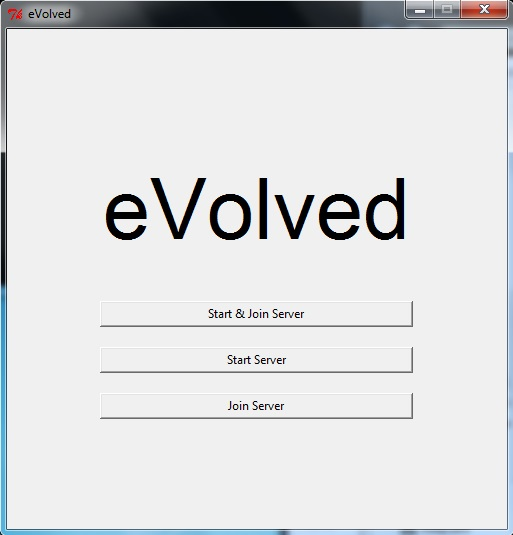
\includegraphics[width=.6\linewidth]{Resources/mainpage}}
}
\end{frame}

\end{document}